\chapter{Theory}
This chapter provides a short and condensed introduction to the theoretical concepts of the methods used in this work. It begins with a discussion of statistical mechanics and free energy techniques, followed by an overview of density functional theory and \textit{ab initio} molecular dynamics. Finally, the chapter concludes with a brief introduction to graph neural networks and neural network potentials. The aim is to provide a comprehensive background to the methods used, while the technical details and derivations are left to the literature sources cited throughout the text.

\section{A brief introduction to statistical mechanics}
The discussion in this section is mostly based on the ``Introduction to Computational Chemistry'' textbook written by Jensen~\citep{jensenIntroductionComputationalChemistry2017}, ``Statistical Mechanics: Theory and Molecular Simulation'' by Tuckermann~\citep{tuckermanStatisticalMechanicsTheory2023}, and ``Understanding Molecular Simulation: From Algorithms to Applications'' by Frenkel and Smit~\citep{frenkelUnderstandingMolecularSimulation2002} unless stated otherwise.



\subsection{Partition functions}
The development of the field of statistical mechanics has been crucial for the computational chemistry community, as it enables the connection between the jigglings and wigglings of atoms and the properties of much larger systems such as liquids and solids.

Let us begin with the most fundamental concept: the partition function. The partition function is akin to a Swiss army knife in statistical mechanics, meaning it is a versatile tool that makes the connection between microscopic and macroscopic properties in thermodynamics possible. In the simplest case of a single molecule, the partition function $q$ takes the following form:

\begin{equation}
    q = \sum_{i = \text{levels}}^{\infty} g_i e^{-\epsilon_i/kT}
\end{equation}

Here, it is expressed as a sum over all energy levels $\epsilon_i$ of a molecule (or particle), multiplied by a degeneracy factor $g_i$ in cases where multiple levels have the same energy. The term $kT$ represents the Boltzmann factor.

Moving on to a more complex scenario in which the partition function describes multiple molecules, we arrive at the partition function $Q$ for non-interacting particles, such as those in an ideal gas:

\begin{equation}
    \label{eq:Q_noninteracting}
    Q = q^N \; \text{(different particles)} \quad Q = \frac{q^N}{N!} \; \text{(identical particles)}
\end{equation}

Here, $N$ denotes the total number of particles. However, one could argue that if we wish to describe a real system such as bulk water, we must account for interactions between molecules. Consequently, Equation~\ref{eq:Q_noninteracting} must be rewritten:

\begin{equation}
    Q = \sum_{i}^{\infty} e^{-E_i/kT}
\end{equation}

In this case, the partition function $Q$ includes contributions from all possible energy states $E_i$ of the system.

Although the concept of the partition function might initially appear abstract, it can be clarified by expressing it in a different form, namely, within the context of the \ac{rrho} approximation, where the electronic, vibrational, and rotational degrees of freedom can be separated. For a single molecule case it would look like:

\begin{equation}
    q_{\text{tot}} = q_{\text{trans}} \times q_{\text{rot}} \times q_{\text{vib}} \times q_{\text{elec}}
\end{equation}

Let us now examine each contribution in more detail. From this point onward we will consider polyatomic molecules in the formulation of the partition functions, unless stated otherwise.

The translational partition function $q_\text{trans}$ can be derived from the energy expression for a particle in a one-dimensional box and is given by:

\begin{equation}
    q_{\text{trans}} = \left(\frac{2\pi MkT}{h^2}\right)^{3/2} V
\end{equation}

Here, $M$ is the total molecular mass, and $V$ is the volume. Turning to the rotational partition function $q_\text{rot}$, it can be derived from the Schr\"odinger equation for a diatomic "rigid rotor" and has the following form:

\begin{equation}
    q_{\text{rot}} = \frac{8\pi^2IkT}{h^2\sigma}
\end{equation}

In this expression, $I$ denotes the moment of inertia, and $\sigma$ represents the symmetry factor, i.e. the order of the rotational subgroup within the molecular point group. For polyatomic molecules, writing an exact expression is more complex, but an approximate form can be used:

\begin{equation}
    q_{\text{rot}} = \frac{\sqrt{\pi}}{\sigma}\left(\frac{8\pi^2kT}{h^2}\right)^{3/2} \sqrt{I_1I_2I_3}
\end{equation}

For the vibrational partition function $q_\text{vib}$, it is expressed as a product over the various vibrational modes of a molecule, each with frequency $\nu_i$:

\begin{equation}
    q_{\text{vib}} = \prod_{i} \frac{e^{-h\nu_i/2kT}}{1-e^{-h\nu_i/kT}}
\end{equation}

Lastly, the electronic partition function $q_\text{elec}$ is given as a sum over all electronic states of a molecule, from the ground state to all excited states. However, since the energy difference between the ground state and higher states is usually much greater than $kT$ at ambient temperatures, the function can typically be approximated by considering only the ground state:

\begin{equation}
    q_{\text{elec}} = \sum_{i=0}^{\infty} g_i e^{-\epsilon_i/kT} \approx g_0 e^{-\epsilon_0/kT}
\end{equation} 



\subsection{Macroscopic properties and thermodynamic functions}

Once the partition function is determined, it provides a direct means of evaluating macroscopic properties. For instance, the internal energy $U$ and the Helmholtz free energy $A$ can be calculated from the partition function $Q$:

\begin{align}
    U &= kT^2 \left(\frac{\partial \ln Q}{\partial T}\right)_V \\
    A &= -kT\ln Q
\end{align}

In addition, other macroscopic properties, such as pressure $P$ and the heat capacity at constant volume $C_V$, can also be expressed in terms of the partition function:

\begin{align}
    P &= -\left(\frac{\partial A}{\partial V}\right)_T = kT\left(\frac{\partial \ln Q}{\partial V}\right)_T \\
    C_V &= \left(\frac{\partial U}{\partial T}\right)_V = 2kT\left(\frac{\partial \ln Q}{\partial T}\right)_V + kT^2\left(\frac{\partial^2 \ln Q}{\partial T^2}\right)_V
\end{align}

Turning to thermodynamic functions, namely enthalpy $H$, entropy $S$, and Gibbs free energy $G$, these can also be derived from the partition function $Q$:

\begin{align}
    H &= U + PV = kT^2\left(\frac{\partial \ln Q}{\partial T}\right)_V + kTV\left(\frac{\partial \ln Q}{\partial V}\right)_T \\
    S &= \frac{U-A}{T} = kT\left(\frac{\partial \ln Q}{\partial T}\right)_V + k\ln Q \\
    G &= H - TS = kTV\left(\frac{\partial \ln Q}{\partial V}\right)_T - kT\ln Q
\end{align}

This connection between macroscopic observables, thermodynamic functions, and the partition function once again highlights its fundamental importance in statistical thermodynamics.



\subsection{The canonical ensemble}
Having established a method to calculate the macroscopic properties of a system we implicitly relied on averaging over a large enough number of states. Therefore one may naturally ask: how can we sample enough configurations to apply the equations described in the previous section under conditions that resemble those in experiments? One such answer is the canonical ensemble.

The canonical ensemble describes a system at constant temperature $T$, fixed volume $V$, and a fixed number of particles $N$ (\acs{nvt}). In this ensemble, the system is in contact with a heat bath, which makes it particularly relevant to most molecular simulations that are describing the experimental conditions, where the temperature is externally controlled while the internal energy of the system is allowed to fluctuate.

Since the energy fluctuates in the canonical ensemble, a logical step is to estimate the magnitude of these fluctuations:

\begin{equation}
    \frac{\Delta E}{E} \sim \frac{\sqrt{N}}{N} \sim \frac{1}{\sqrt{N}}
\end{equation}

Here, $N$ denotes the number of particles, and thus for sufficiently large systems, the relative energy fluctuations become negligible.

The use of the canonical ensemble implicitly assumes that the system is ergodic, meaning that time averages obtained from simulation trajectories are equivalent to ensemble averages over the Boltzmann distribution. This assumption is, for instance, central to molecular dynamics simulations where the canonical ensemble can be sampled.



\subsection{Classical forcefields and molecular dynamics}
Bringing all the puzzle pieces together, we can now discuss how to simulate a molecular or atomic system of interest. One widely used approach is \ac{md} simulations. The first step involves defining a potential energy function that describes the interactions between atoms. This function, often referred to as a forcefield, is typically parameterised based on experimental data or high-level quantum mechanical calculations.

In classical \ac{md}, the evolution of a system of $N$ atoms is governed by Newton's equations of motion. A commonly used form of the potential energy function is:

\begin{equation}
\begin{aligned}
    U(\mathbf{r}_1, \dots, \mathbf{r}_N) = &\sum_{\text{bonds}} \frac{1}{2} K_{\text{bond}} (r - r_0)^2 + 
    \sum_{\text{bends}} \frac{1}{2} K_{\text{bend}} (\theta - \theta_0)^2 \\
    &+ \sum_{\text{tors}} \sum_{n=0}^{6} A_n \left[ 1 + \cos(C_n \phi + \delta_n) \right] \\
    &+ \sum_{i,j \in \text{nb}} \left\{ \left[ 4\epsilon_{ij} \left( \frac{\sigma_{ij}}{r_{ij}} \right)^{12}
    - \left( \frac{\sigma_{ij}}{r_{ij}} \right)^6 \right] + \frac{q_i q_j}{r_{ij}} \right\}
\end{aligned}
\label{eq:md_potential}
\end{equation}

Here, the total energy is decomposed into bonded interactions (bonds, angles, and torsions) and non-bonded interactions, including Lennard-Jones and Coulombic terms. Once the potential is specified, the force on each atom $i$ is obtained via:

\begin{equation}
    \mathbf{F}_i = -\frac{\partial U}{\partial \mathbf{r}_i}
    \label{eq:md_force}
\end{equation}

To propagate the positions and velocities of atoms in time, numerical integration schemes are employed. Among these, the velocity Verlet algorithm is widely used in perhaps all \ac{md} engines. Let us consider the Taylor expansion of the position of particle $i$ to second order in the time step $\Delta t$:

\begin{equation}
    \mathbf{r}_i(t + \Delta t) \approx \mathbf{r}_i(t) + \Delta t\, \mathbf{v}_i(t) + \frac{\Delta t^2}{2m_i} \mathbf{F}_i(t)
    \label{eq:vv_pos}
\end{equation}

Here, $\mathbf{F}_i(t)$ is the force on particle $i$ at time $t$, and $m_i$ is its mass, calculated using Equation~\ref{eq:md_force} and $\mathbf{v}_i(t)$ is its velocity. This expression provides a prediction of the new position based on the current velocity and force.

We can also consider a backward expansion in time from $\mathbf{r}_i(t + \Delta t)$ and $\mathbf{v}_i(t + \Delta t)$, yielding:

\begin{equation}
    \mathbf{r}_i(t) = \mathbf{r}_i(t + \Delta t) - \Delta t\, \mathbf{v}_i(t + \Delta t) + \frac{\Delta t^2}{2m_i} \mathbf{F}_i(t + \Delta t)
    \label{eq:vv_pos_backward}
\end{equation}

By substituting Equation~\ref{eq:vv_pos} into Equation~\ref{eq:vv_pos_backward} and solving for $\mathbf{v}_i(t + \Delta t)$, we get:

\begin{equation}
    \mathbf{v}_i(t + \Delta t) = \mathbf{v}_i(t) + \frac{\Delta t}{2m_i} \left[ \mathbf{F}_i(t) + \mathbf{F}_i(t + \Delta t) \right]
    \label{eq:vv_vel}
\end{equation}

Equations~\ref{eq:vv_pos} and \ref{eq:vv_vel} together form the velocity Verlet integrator. The algorithm proceeds as follows:
\begin{enumerate}
  \item First, update positions using Equation~\ref{eq:vv_pos}.
  \item Then, compute new forces $\mathbf{F}_i(t + \Delta t)$ based on the updated positions.
  \item Finally, update velocities using Equation~\ref{eq:vv_vel}.
\end{enumerate}

To correctly sample the canonical ensemble, one should consider the use of thermostats to maintain the system temperature. In this work, we focus on two widely used thermostats: the Nos\'e--Hoover thermostat~\citep{noseUnifiedFormulationConstant1984, hooverCanonicalDynamicsEquilibrium1985} and the \ac{csvr} thermostat~\citep{bussiCanonicalSamplingVelocity2007}. In the former, the equations of motion are modified to include a friction term that couples the system to a heat bath, allowing for energy exchange. The \ac{csvr} thermostat, on the other hand, uses a velocity rescaling approach to maintain the desired temperature by adjusting particle velocities at each time step.



\subsection{Enhanced sampling techniques}
Even though \ac{md} simulations are a powerful tool for studying molecular systems, their applicability can be limited due to the presence of energy barriers separating minima in the potential energy landscape. As a result, the system may remain trapped in local minima, leading to insufficient sampling of the relevant configurational space. This issue becomes particularly pronounced in the context of reactive systems, where rare events involve transitions between states separated by high free energy barriers and occur on timescales much longer than typical simulation durations.

To address this challenge, various enhanced sampling techniques have been developed. These methods aim to accelerate the exploration of phase space. In general, they bias the system along reaction coordinates, or \acp{cv}, by applying a biasing potential that drives the system towards regions of interest. One such approach is metadynamics~\citep{laioEscapingFreeenergyMinima2002, laioMetadynamicsMethodSimulate2008}.

In metadynamics, a biasing (external) potential is added to the system's potential energy surface. This biasing potential takes the following form:

\begin{equation}
    V(S(x), t) = w \sum_{t' = \tau_{\text{G}}, 2\tau_{\text{G}}, \ldots}^{t' < t} \exp\left(-\frac{(S(x) - s(t'))^2}{2\delta s^2}\right)
    \label{eq:biasing_potential}
\end{equation}

where $s(t) = S(x(t))$ is the value of the \ac{cv} at time $t$. The height of the Gaussian kernel is denoted by $w$, $\delta s$ is its width, and $\tau_{\text{G}}$ is the deposition rate.

The approach used in metadynamics can be explained using the Panama Canal as an analogy as illustrated in Figure~\ref{fig:metadynamics}. The idea is to fill the basins of the free energy landscape with a Gaussian potential, which can be thought of as water gradually filling the basins, lifting the system (like a ship in a lock) out of a free energy minimum and helping it traverse to other states.

The assumption in metadynamics is that, after sufficiently long sampling, the biasing potential $V_{\text{G}}(S, t)$ converges to the negative of the underlying free energy surface:

\begin{equation}
    \label{eq:free_energy_from_metadynamics}
    \lim_{t \to \infty} V(s,t) \sim -F(s)
\end{equation}

Despite the many benefits that metadynamics offers, it is important to note that it has limitations. For example, obtaining a converged free energy surface is not straightforward, especially when multiple \acp{cv} are involved. In principle, Gaussian kernels can be deposited indefinitely, making it difficult to assess convergence. To address this issue, the well-tempered variant of metadynamics was developed~\citep{barducciWellTemperedMetadynamicsSmoothly2008}. In this method, a history-dependent potential is added, which is defined as:

\begin{equation}
    V(s, t) = \Delta T \ln\left(1 + \frac{\omega N(s, t)}{\Delta T}\right)
    \label{eq:history_dependant_potential}
\end{equation}

Here, $N(s, t)$ is the histogram of $s$ obtained from a biased simulation, $\Delta T$ is the biasing temperature, and $\omega$ has the dimension of an energy rate. The rate at which this potential is modified over time is given by:

\begin{figure}[t!]
    \centering
    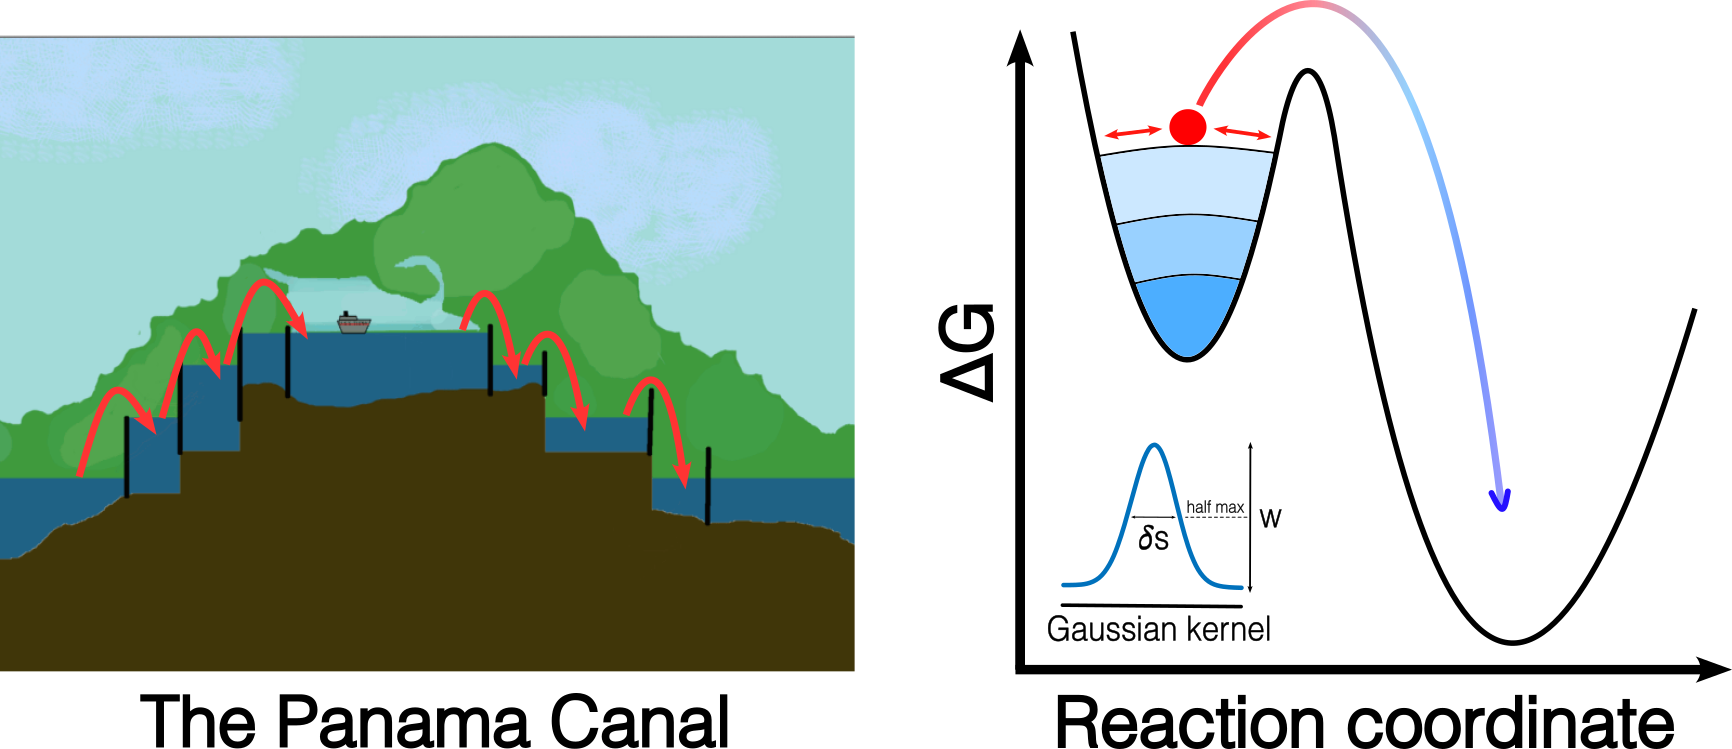
\includegraphics[width=0.8\textwidth]{Figures/2_Theory/theory_metadynamics.png}
    \caption{The concept of metadynamics. $w$ stands for the Gaussian kernel height, and $\delta s$ stands for its width. The Panama Canal cartoon was taken from~\citep{HowPanamaCanal}.}
    \label{fig:metadynamics}
\end{figure}

\begin{equation}
    \dot{V}(s,t) = \frac{\omega \Delta T \delta_{s,s(t)}}{\Delta T + \omega N(s,t)} 
    = \omega e^{-[V(s,t)/\Delta T]} \delta_{s,s(t)}
    \label{eq:hill_deposition_rate}
\end{equation}

The height of the Gaussian kernels used is:

\begin{equation}
    w = \omega e^{-[V(s,t)/\Delta T]} \tau_{\text{G}}
    \label{eq:hill_height}
\end{equation}

where $\tau_{\text{G}}$ is the deposition rate and $\omega$ represents the initial bias deposition rate. The Gaussian kernel height is now dependent on the history of the system, allowing for a more controlled exploration of the free energy landscape.

Ultimately, the underlying free energy surface can be estimated using the following equation:

\begin{equation}
    \tilde{F}(s,t) = -\frac{T + \Delta T}{\Delta T} V(s,t) 
    = -(T + \Delta T) \ln\left(1 + \frac{\omega N(s,t)}{\Delta T} \right)
    \label{eq:free_energy_surface_reconstruction}
\end{equation}

The advantage of \ac{wtmd} is that it enables more efficient exploration of the free energy landscape, as the biasing potential adapts according to the trajectory's history. Moreover, the convergence can be easily monitored by observing the decay of the Gaussian height, which should approach zero as the system fully explores the relevant phase space.



%%%%%%%%%%%%%%%%%%%%%%%%%%%%%%%%%%%%%%%%%%%%%%%%%%%%%%%%%%%%%%%%%%%%%%%%%%%%%%%%

% \section{Transition state theory}



%%%%%%%%%%%%%%%%%%%%%%%%%%%%%%%%%%%%%%%%%%%%%%%%%%%%%%%%%%%%%%%%%%%%%%%%%%%%%%%%

\section{The density functional theory tourist}
The discussion in this section is primarily based on the ``Introduction to Computational Chemistry'' textbook written by Jensen~\citep{jensenIntroductionComputationalChemistry2017}, ``Density Functional Theory: a Practical Introduction'' by Scholl and Steckel~\citep{shollDensityFunctionalTheory2011}, and ``A Chemist's Guide to Density Functional Theory'' by Koch and Holthausen~\citep{kochChemistsGuideDensity2015} unless stated otherwise.

\subsection{The Kohn-Sham approach}
In order to describe reactive events in relatively large systems, up to approximately 1,000 atoms, it is necessary to use methods that offer a good balance between accuracy and computational cost. One such method is \ac{dft}, which is based on the Hohenberg-Kohn theorems and the Kohn-Sham equations.

The central idea behind \ac{dft}, established by Hohenberg and Kohn, is that the ground state energy of a many-electron system can be expressed as a functional of the electron density. This reformulation reduces the problem from solving a 3$N$-dimensional wavefunction to working with a 3-dimensional electron density.

The energy functional can be written as:

\begin{equation}
    \begin{aligned}
    E[\rho(\mathbf{r})] &= T_{\text{s}}[\rho] + J[\rho] + E_{\text{Ne}}[\rho] + E_{\text{XC}}[\rho] =  \\
    &= -\frac{1}{2} \sum_{i}^{N} \langle \phi_i | \nabla^2 | \phi_i \rangle \\
    &\quad + \frac{1}{2} \sum_{i}^{N} \sum_{j}^{N} \iint \left| \phi_i(\mathbf{r}_1) \right|^2 \frac{1}{r_{12}} \left| \phi_j(\mathbf{r}_2) \right|^2 d\mathbf{r}_1 d\mathbf{r}_2 \\
    &\quad - \sum_{i}^{N} \sum_{A}^{M} \int \frac{Z_A}{r_{1A}} \left| \phi_i(\mathbf{r}_1) \right|^2 d\mathbf{r}_1 \\
    &\quad + E_{\text{XC}}[\rho(\mathbf{r})] 
    \label{eq:ks_energy}
    \end{aligned}
\end{equation}

Here, the first three terms are “known” and represent the kinetic energy of the electrons, the Coulomb interaction between the electrons, and the electron-nucleus interaction, respectively. The final term, the exchange-correlation energy functional, is the unknown component. It contains all the effects that are not straightforward to treat exactly, for instance, the residual part of the kinetic energy and the non-classical electron-electron interactions:

\begin{equation}
    E_{\text{XC}}[\rho] \equiv (T[\rho] - T_{\text{s}}[\rho]) + (E_{\text{ee}}[\rho] - J[\rho])
    \label{eq:xc_energy}
\end{equation}

The biggest challenge in \ac{dft} lies in the formulation of $E_{\text{XC}}$. This term is particularly important, as finding the minimum of the total energy functional, as expressed in Equation~\ref{eq:ks_energy}, depends on its accurate representation.

To address this, the Kohn-Sham approach introduces a set of single-electron equations that can be solved iteratively to obtain the electron density and the total energy of the system. The Kohn-Sham equations are given by:

\begin{equation}
    \left( -\frac{1}{2} \nabla^2 + V_{\text{eff}}(\mathbf{r}) \right) \phi_i = \varepsilon_i \phi_i
    \label{eq:ks_equations}
\end{equation}

Here, $V_{\text{eff}}$ takes the form:

\begin{equation}
    V_{\text{eff}}(\mathbf{r}) = \int \frac{\rho(\mathbf{r}_2)}{r_{12}} d\mathbf{r}_2 + V_{\text{XC}}(\mathbf{r}) - \sum_{A}^{M} \frac{Z_A}{r_{1A}}
    \label{eq:v_eff}
\end{equation}

The iterative procedure to solve these equations proceeds as follows: first, a trial electron density is defined. Then, the Kohn-Sham equations are solved using this trial density to obtain the single-particle wavefunctions. Next, a new electron density is calculated from the obtained wavefunctions. Finally, the new density is compared with the initial trial density. If the two densities match within a given convergence criterion, the ground state electron density has been found, and the total energy of the system can be computed.



\subsection{Generalised gradient approximation and PBE functional}

\begin{figure}[t!]
    \centering
    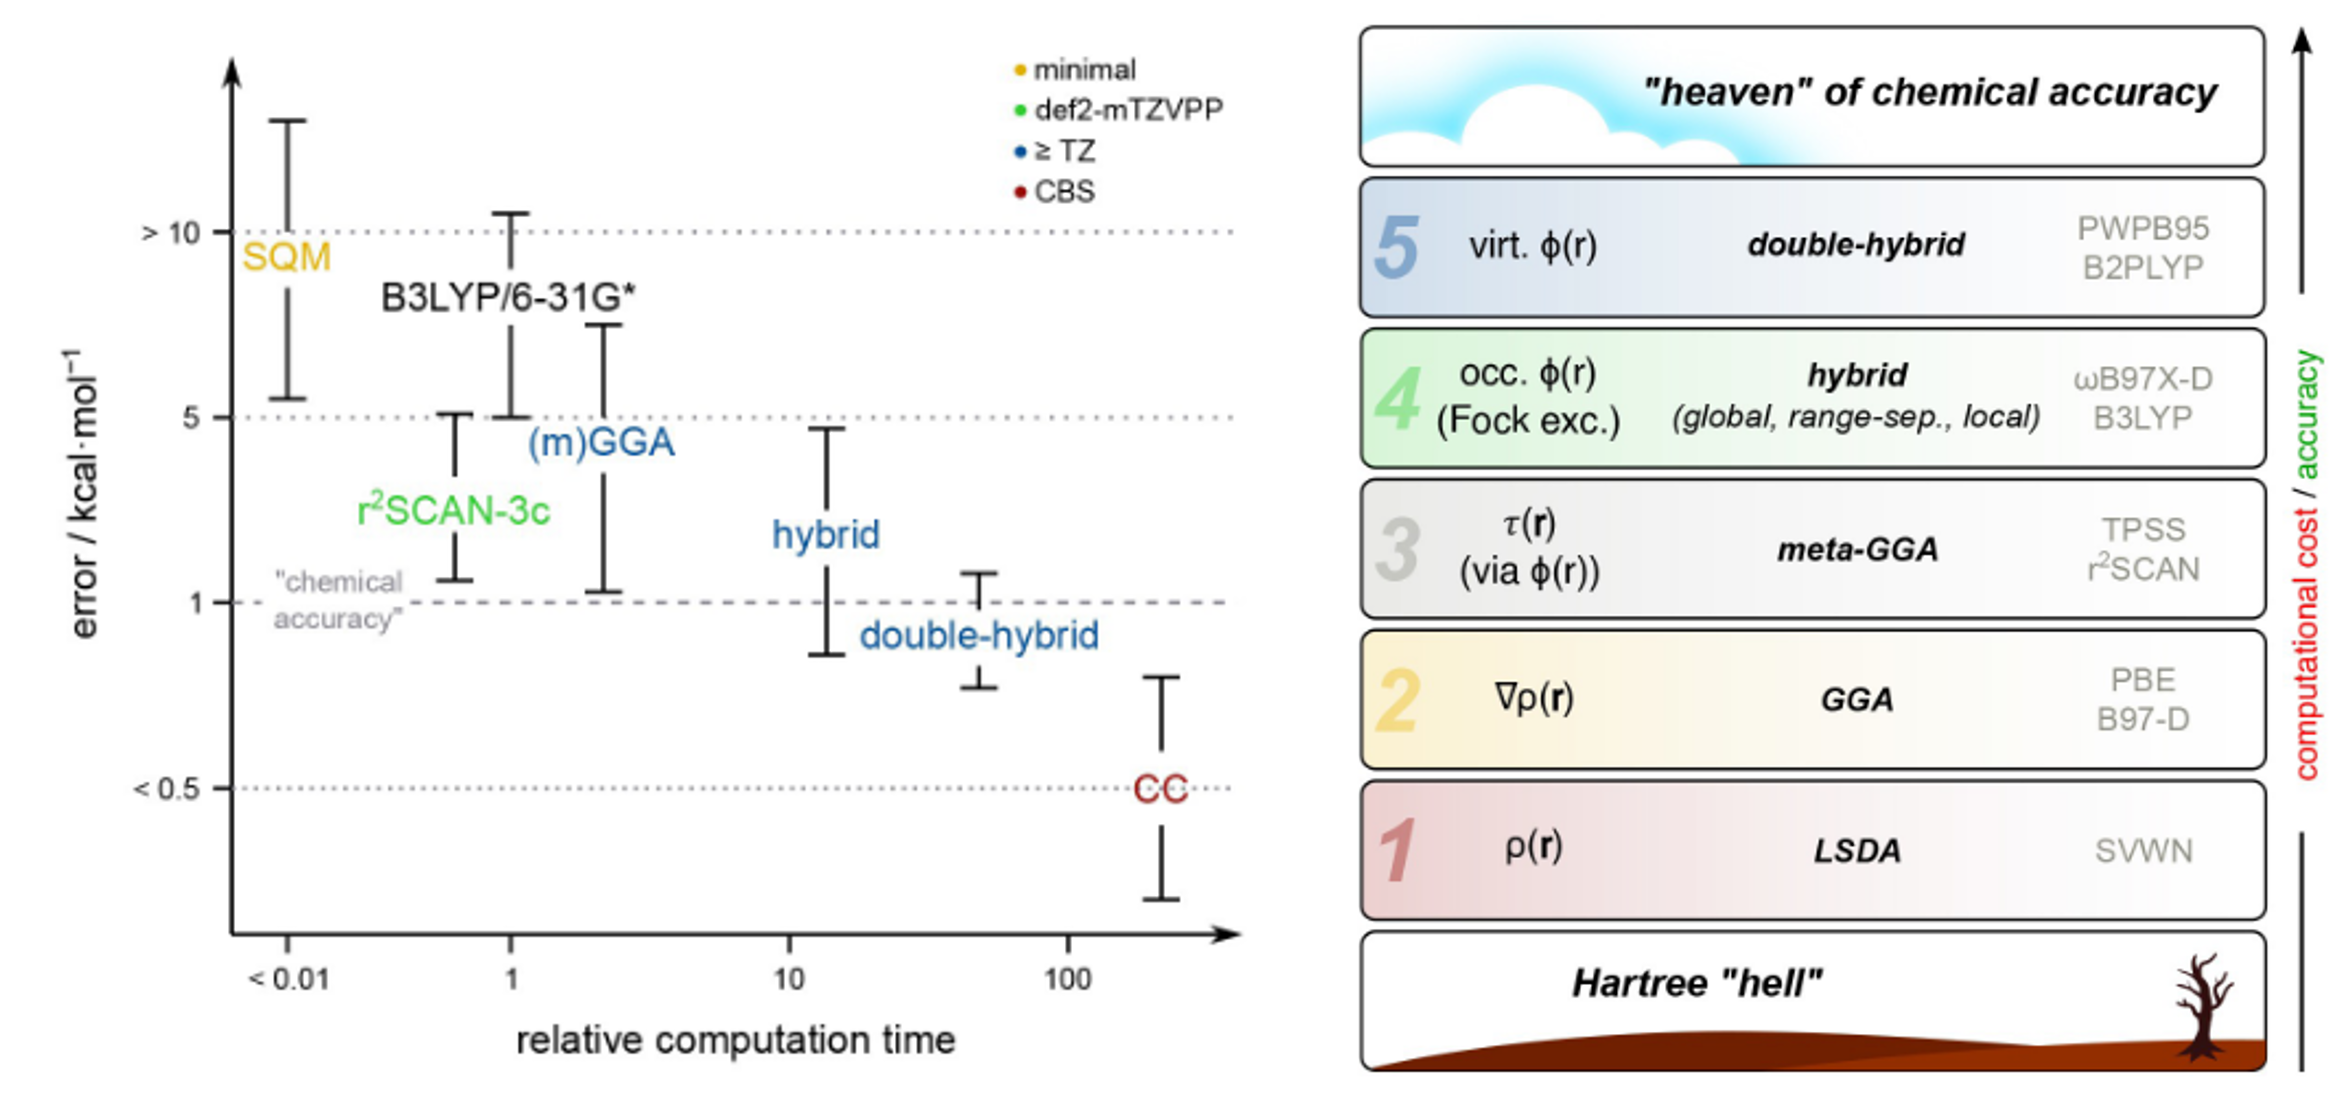
\includegraphics[width=0.7\textwidth]{Figures/2_Theory/theory_jacobs_ladder.png}
    \caption{Left panel: accuracy of the common quantum chemical methods as a function of the computatinal cost. Right panel: categorisation of the exchange-correlation functionals according to Perdew's ``Jacob's ladder''. The figure was reproduced from \citep{burschBestPracticeDFTProtocols2022}.}
    \label{fig:jacobs_ladder}
\end{figure}

The field of \ac{dft} has opened new avenues for computational chemists and physicists, enabling them to study the properties of materials and molecules, as well as to investigate the reaction pathways of chemical processes. However, the accuracy of \ac{dft} calculations is highly dependent on the choice of the exchange-correlation functional.

In this work, we focus on the \ac{gga} exchange-correlation functionals, which are widely used in \ac{dft} calculations and are known to provide results close to chemical accuracy at a relatively low computational cost, as can be seen in Figure~\ref{fig:jacobs_ladder}. In fact, the development of \ac{gga} functionals marked a turning point in the acceptance of the \ac{dft} method by the quantum chemistry community.

The \ac{gga} functionals are based on the idea that the exchange-correlation energy can be expressed as a functional of the electron density $\rho$ and its gradient $\nabla \rho$. The general form of a \ac{gga} functional is given by:

\begin{equation}
E_{\text{XC}}^{\text{GGA}}[\rho] = \int f(\rho, \nabla\rho) \, d\mathbf{r}
\label{eq:gga_functional}
\end{equation}

The exchange-correlation energy can be explicitly divided into two parts:

\begin{equation}
E_{\text{XC}}^{\text{GGA}} = E_{\text{X}}^{\text{GGA}} + E_{\text{C}}^{\text{GGA}}
\label{eq:gga_xc}
\end{equation}

One of the most widely used \ac{gga} functionals is the Perdew-Burke-Ernzerhof (PBE) functional~\citep{perdewGeneralizedGradientApproximation1996}. Its formulation incorporates 4 parameters in the exchange and correlation parts derived from first principles, making it a truly \textit{ab initio} functional.



\subsection{\textit{Ab initio} molecular dynamics}
In one of the previous sections, we touched upon the topic of classical \ac{md} simulations. However, classical force fields are unable to simulate bond-breaking and bond-forming processes. Although reactive events can also be studied using static approaches, by calculating the potential energy surface at a given set of coordinates, we believe that incorporating dynamics provides more informative insights and a clearer picture of the reaction mechanism.

To simulate the dynamics of a chemical reaction, one could consider using \ac{aimd}, and in particular, \ac{bomd}. In \ac{bomd}, the forces acting on the atoms are calculated at each time step using quantum mechanical methods, such as \ac{dft}, while the nuclei are propagated according to classical mechanics. This process can be described using the Lagrangian formalism, $L$, which offers an alternative formulation of classical dynamics:

\begin{equation}
    L = K - U = \frac{1}{2} \sum_{i=1}^{3N} m_i v_i^2 - E[\phi(\mathbf{r}_1, \ldots, \mathbf{r}_{3N})]
    \label{eq:lagrangian_aimd}
\end{equation}

where $K$ is the kinetic energy, $U$ represents the potential energy, and $\phi(\mathbf{r}_1, \ldots, \mathbf{r}_{3N})$ is a set of one-electron Kohn-Sham wave functions.

It is important to note that, since nuclear dynamics are treated classically in this framework, zero-point vibrational energy is not accounted for, nor can tunnelling effects be studied. 



%%%%%%%%%%%%%%%%%%%%%%%%%%%%%%%%%%%%%%%%%%%%%%%%%%%%%%%%%%%%%%%%%%%%%%%%%%%%%%%%

\section{Extended tight binding}
The tight binding methods can be viewed as a simplification, or semi-empirical approximation, of \ac{dft}. Essentially, they are based on the same principles but introduce numerous approximations to reduce the computational cost. In 2017, the \ac{xtb} method was introduced. This development led to a new family of methods, namely GFNn-xTB, where GFN stands for geometries, frequencies, and non-covalent interactions, and \emph{n} denotes the version~\citep{grimmeRobustAccurateTightBinding2017}.

In \ac{dftb} methods, the total energy of a system is expressed as a Taylor expansion around $\Delta \rho$~\citep{bannwarthExtendedTightbindingQuantum2021}:

\begin{equation}
    E[\rho] = E^{(0)}[\rho_0] + E^{(1)}[\rho_0, \delta \rho] + E^{(2)}[\rho_0, (\delta \rho)^2] + E^{(3)}[\rho_0, (\delta \rho)^3] + \cdots
    \label{eq:tb_energy_expansion}
\end{equation}

Here, $\Delta \rho$ represents the difference between the converged $\rho$ and the reference density $\rho_0$. The terms represent zeroth-order (core-core repulsion), first-order (valence electronic energy), second-order (charge corrections), and higher-order terms~\citep{jensenIntroductionComputationalChemistry2017}. GFNn-xTB is heavily based on \ac{dftb}3, which includes terms in the energy expansion up to third order. The energy of GFN1-xTB, which is considered in this work, is given by~\citep{bannwarthExtendedTightbindingQuantum2021}:

\begin{equation}
    \begin{aligned}
    E_{\text{GFN1-xTB}} &= E_{\text{rep}}^{(0)} + E_{\text{disp}}^{(0)} + E_{\text{XB}}^{(0)} + E_{\text{EHT}}^{(1)} + E_{\text{IES+IXC}}^{(2)} + E_{\text{IES+IXC}}^{(3)} \\
    &= E_{\text{rep}} + E_{\text{disp}}^{\text{D3}} + E_{\text{XB}}^{\text{GFN1}} + E_{\text{EHT}} + E_{\gamma} + E_{\Gamma}^{\text{GFN1}}
    \end{aligned}
    \label{eq:gfn1xtb_energy}
\end{equation}

where $E_{\text{rep}}$ is the repulsion energy, $E_{\text{disp}}^{\text{D3}}$ is the dispersion energy, $E_{\text{XB}}^{\text{GFN1}}$ is the exchange-bonding energy, $E_{\text{EHT}}$ is the extended H\"uckel theory energy, and $E_\gamma$ and $E_\Gamma^{\text{GFN1}}$ correspond to contributions arising from density fluctuations.

It is important to note that the GFNn-xTB methods are parametrised for 86 elements using a partially polarised minimal valence basis set. GFN1-xTB provides a good first approximation of the potential energy surface and is computationally efficient, thus making it suitable for the initial exploration of large molecular systems and running relatively long \ac{md} simulations.


%%%%%%%%%%%%%%%%%%%%%%%%%%%%%%%%%%%%%%%%%%%%%%%%%%%%%%%%%%%%%%%%%%%%%%%%%%%%%%%%
\section{Neural network potentials}
The discussion in this section is mainly based on the textbook ``Deep Learning: Foundations and Concepts'' by C. M. Bishop and H. Bishop~\citep{bishopDeepLearningFoundations2023}, the excellent review by Duval, Mathis, Joshi, and Schmidt et al.~\citep{duvalHitchhikersGuideGeometric2024}, the research paper by Batatia and Batzner et al.~\citep{batatiaDesignSpaceE3Equivariant2022}, and the research paper by Batzner et al.~\citep{batznerE3equivariantGraphNeural2022}, unless stated otherwise.

\subsection{Graph neural networks}
One can easily imagine how computationally expensive it would be to run \ac{aimd} simulations for a system containing hundreds of atoms. In recent years, the field of machine learning has made significant progress in addressing this challenge. In particular, the development of \acp{gnn} has enabled the design of \acp{nnp}, which learn the potential energy surface of molecular systems and can replace \ac{dft} in molecular dynamics simulations.

A natural question one may ask here: why use \acp{gnn}? The answer lies in the fact that \acp{gnn} provide a natural way to represent molecular systems. Atoms can be considered as nodes in a graph, with bonds between them represented as edges. This concept is visualised in Figure~\ref{fig:graph_and_geometric_nns}~A.

\begin{figure}[t!]
    \centering
    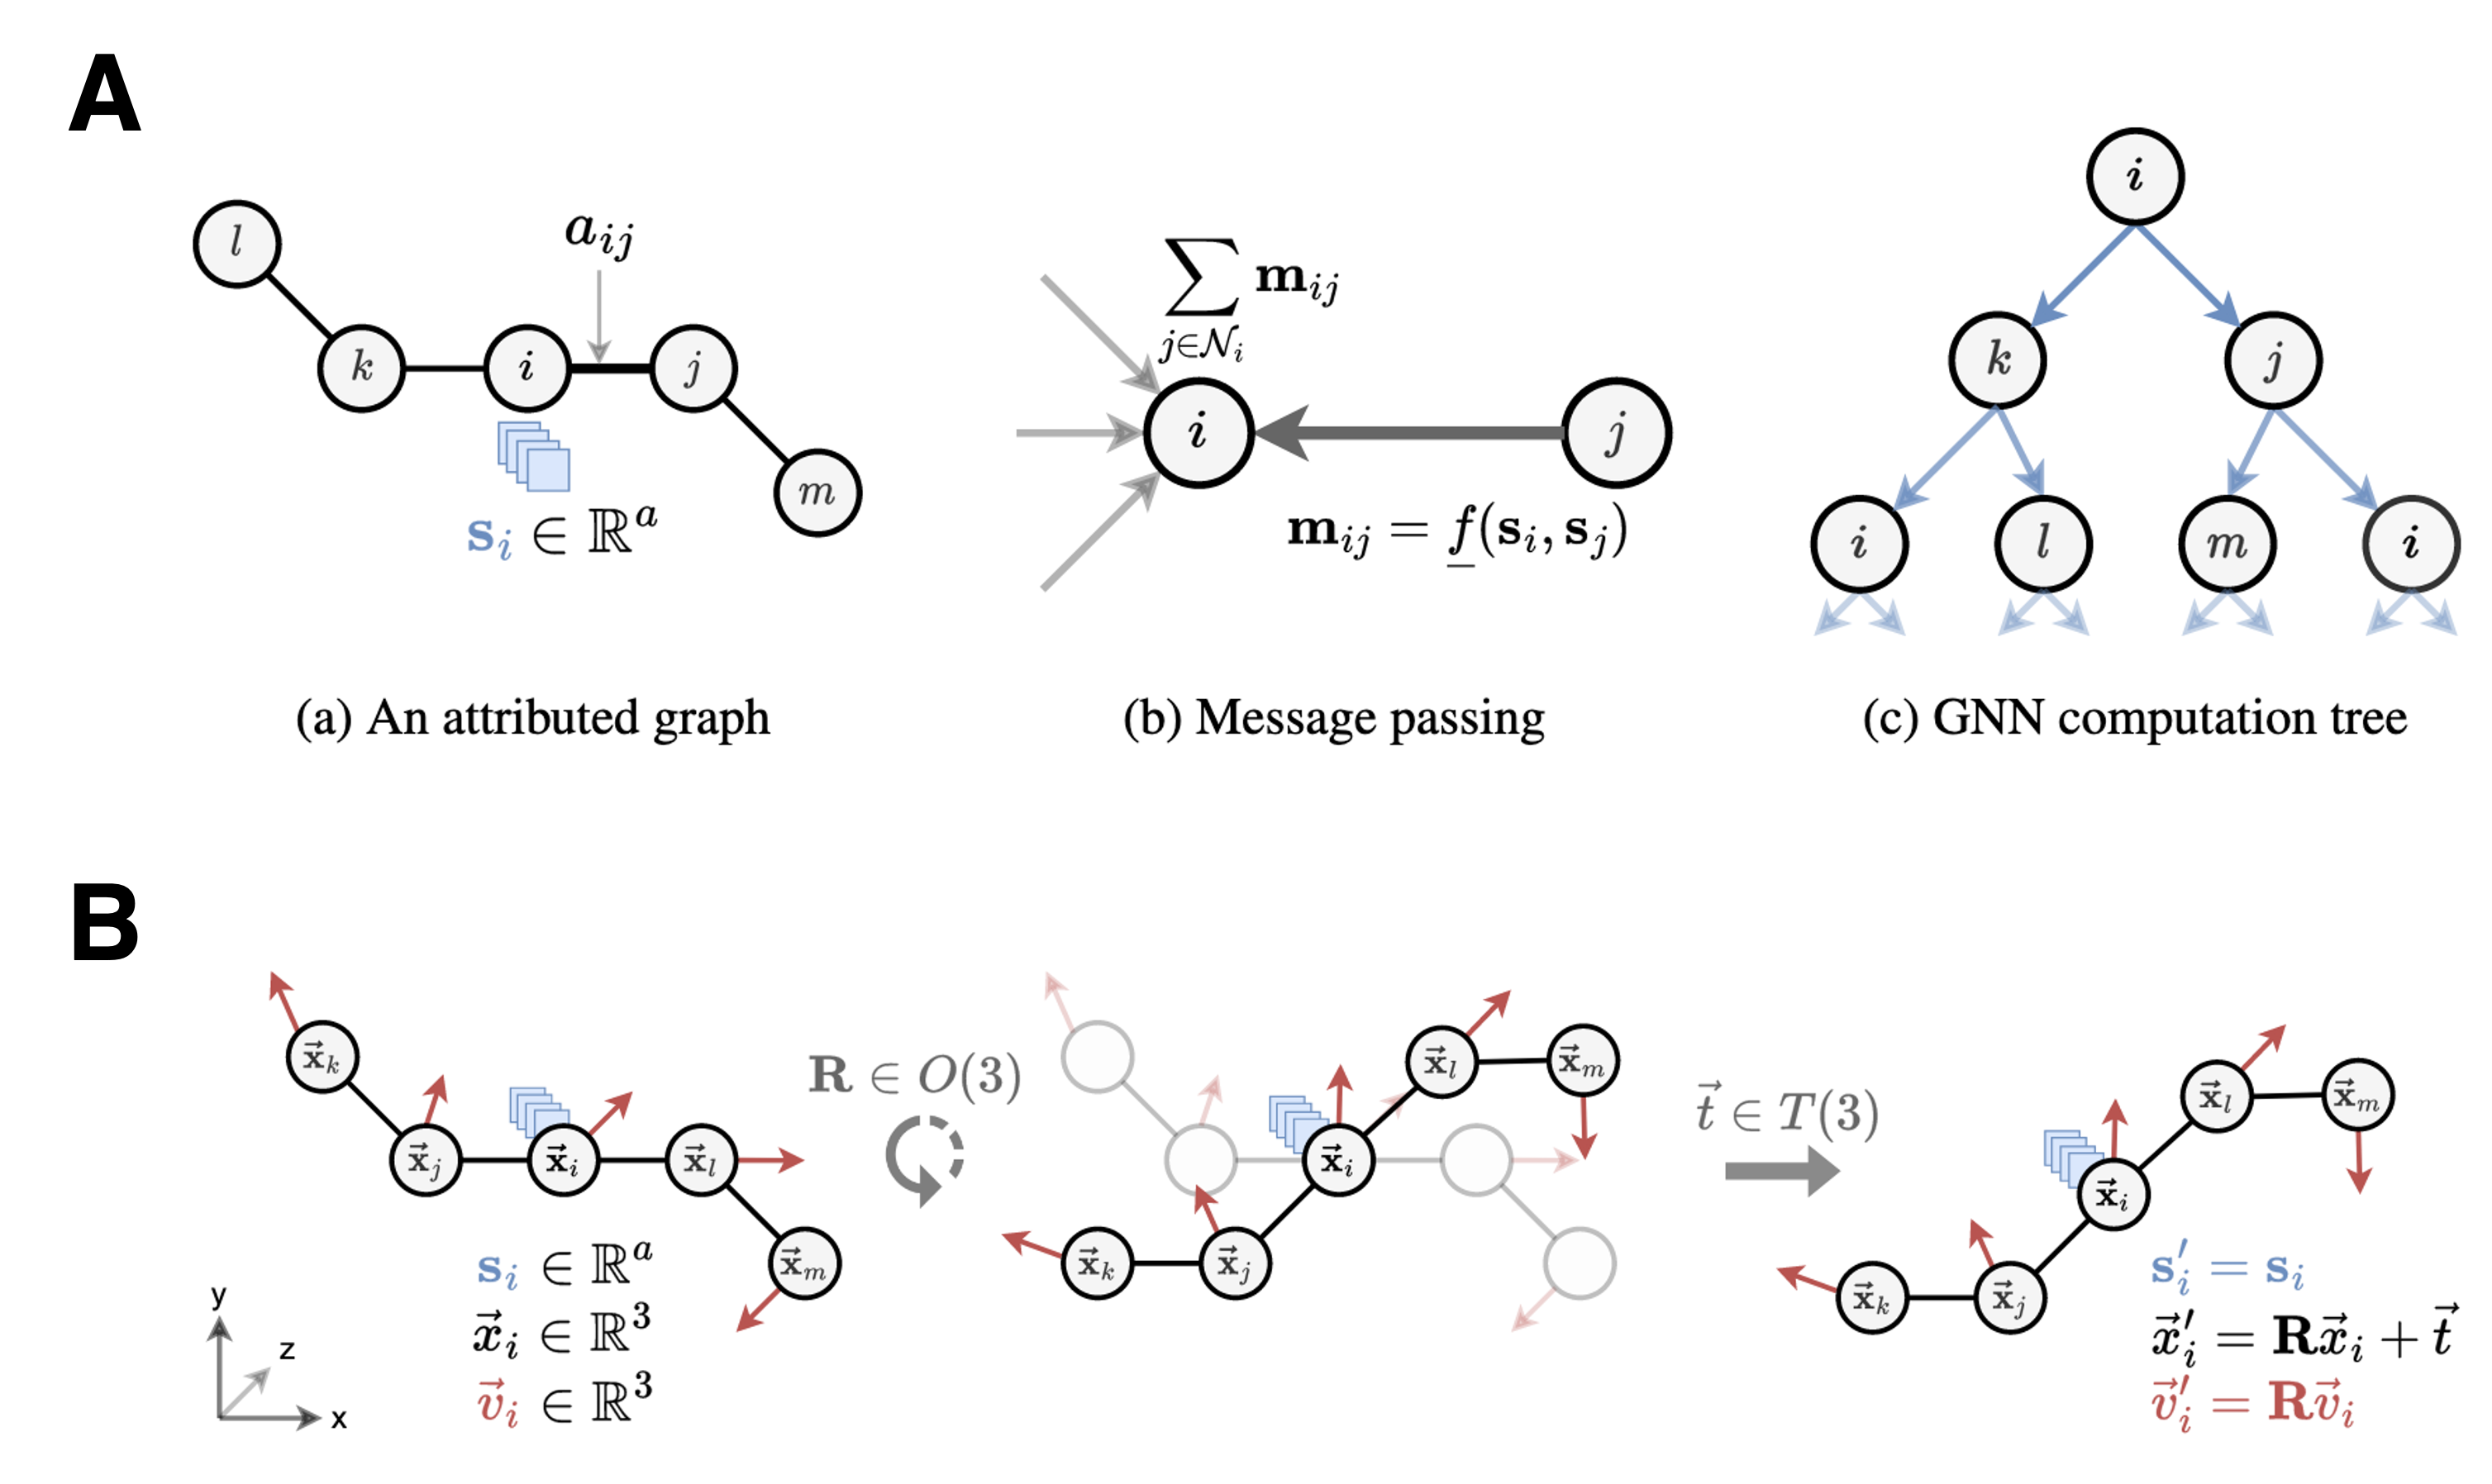
\includegraphics[width=0.7\textwidth]{Figures/2_Theory/graph_and_geometric_nns.png}
    \caption{The concept of (A) \acp{gnn} and (B) geometric \acp{gnn} visualised. This figure was reproduced from \citep{duvalHitchhikersGuideGeometric2024}.}
    \label{fig:graph_and_geometric_nns}
\end{figure}

An essential property of any graph $\mathcal{G} = (\mathbf{A}, \mathbf{S})$ is its adjacency matrix $\mathbf{A}$, which encodes the connectivity of the nodes via elements $a_{ij}$. This matrix is square with dimensions $n \times n$, where $n$ is the number of nodes in the graph. Each entry is either 0 or 1, indicating the absence or presence of a connection between two nodes.

Because the ordering of nodes in the graph is arbitrary, \acp{gnn} are, by construction, permutation symmetric.

In addition to the adjacency matrix, each graph also has a matrix of scalar features $\mathbf{S}$ associated with its nodes. In the case of molecular systems, these features may include atomic numbers or atom types.

\Acp{gnn} are neural networks specifically designed to operate on graph-structured data. They learn representations of nodes, edges, or entire graphs by iteratively updating node features based on their neighbours $\mathcal{N}_i$. This iterative process is commonly referred to as message passing, illustrated in Figure~\ref{fig:graph_and_geometric_nns}~A. Conceptually, the process proceeds as follows:
\begin{enumerate}
    \item At iteration $t$, each node $i$ receives messages from its neighbours $\mathcal{N}_i$:
    \begin{equation}
        \mathbf{m}_{ij}^{(t)} = \underline{\text{MSG}}\left(\mathbf{s}_i^{(t)}, \mathbf{s}_j^{(t)}\right)
        \label{eq:message_passing}
    \end{equation}

    \item These messages are aggregated to update the node's features: $\bigoplus_{j \in \mathcal{N}_i} \mathbf{m}_{ij}^{(t)}$.
        
    \item At iteration $t + 1$, the node's representation is updated using the aggregated messages and its current state:
    \begin{equation}
        \mathbf{s}_i^{(t+1)} = \underline{\text{UPD}}\left(\mathbf{s}_i^{(t)}, \bigoplus_{j \in \mathcal{N}_i} \mathbf{m}_{ij}^{(t)}\right)
        \label{eq:representation_update}
    \end{equation}
\end{enumerate}

The $\underline{\text{MSG}}$ and $\underline{\text{UPD}}$ functions form an entire research topic within \acp{gnn}, and are typically implemented as neural networks themselves. The aggregation operator $\bigoplus$ must be permutation-invariant and can take forms such as summation, averaging, etc. After the final iteration, the resulting node representations can be used to predict properties at various levels, whether for the entire graph, such as the total energy of a molecular system, or at the node or edge level.

A particularly important subclass of \acp{gnn} is the geometric \acp{gnn}, which are designed to handle geometric data in Euclidean space. These are depicted in Figure~\ref{fig:graph_and_geometric_nns}~B. Geometric graphs $\mathcal{G} = (\mathbf{A}, \mathbf{S}, \vec{\mathbf{x}}, \vec{\mathbf{v}})$ contain additional information such as atomic coordinates $\vec{x_i}$ and other vector features $\vec{v_i}$. These vectors may represent quantities such as velocities or forces.

Geometric \acp{gnn} are tailored to work with data that has an inherent geometric structure, such as point clouds. Their key advantage is in handling symmetry operations, i.e. that under rotations and translations of the data, scalar features remain invariant, or the same, while vector features transform appropriately. This property is crucial for accurately capturing the underlying physics of molecular systems.



\subsection{Invariance and equivariance}

In the context of geometric \acp{gnn}, the concepts of invariance and equivariance play a fundamental role in ensuring that models respect the symmetries of the data they are trained on. These properties are especially crucial when working with molecules, where rotations or translations should not change the outcome of the prediction or should change it in a predictable way.

Mathematically, a function $f$ is said to be invariant to a transformation $g$ if applying $g$ to the input $x$ does not affect the output of the function:

\begin{equation}
f(g \cdot x) = f(x)
\label{eq:invariance}
\end{equation}

A simple real-world example of invariance is the total energy of a molecule. Typically it stays invariant under rotations and translations of its atomic coordinates.

On the other hand, a function $f$ is said to be equivariant to a transformation $g$ if applying $g$ to the input results in the same transformation being applied to the output:

\begin{equation}
f(g \cdot x) = g \cdot f(x)
\label{eq:equivariance}
\end{equation}

A familiar example of equivariance is the behaviour of vector quantities such as velocity or force. If we rotate a coordinate system (or the object within it), the velocity or force vectors will also rotate accordingly. In the context of molecular systems, atomic forces are equivariant under rotations: if the molecule is rotated, the directions of the forces rotate in the same way. Both concepts of invariance and equivariance are illustrated in Figure~\ref{fig:invariance_equivariance}.

Designing \acp{gnn} that are invariant or equivariant helps reduce the amount of data needed for training. Geometric neural networks, for instance, are explicitly constructed to respect such symmetries, making them particularly well-suited for chemical modelling.

\begin{figure}[t!]
    \centering
    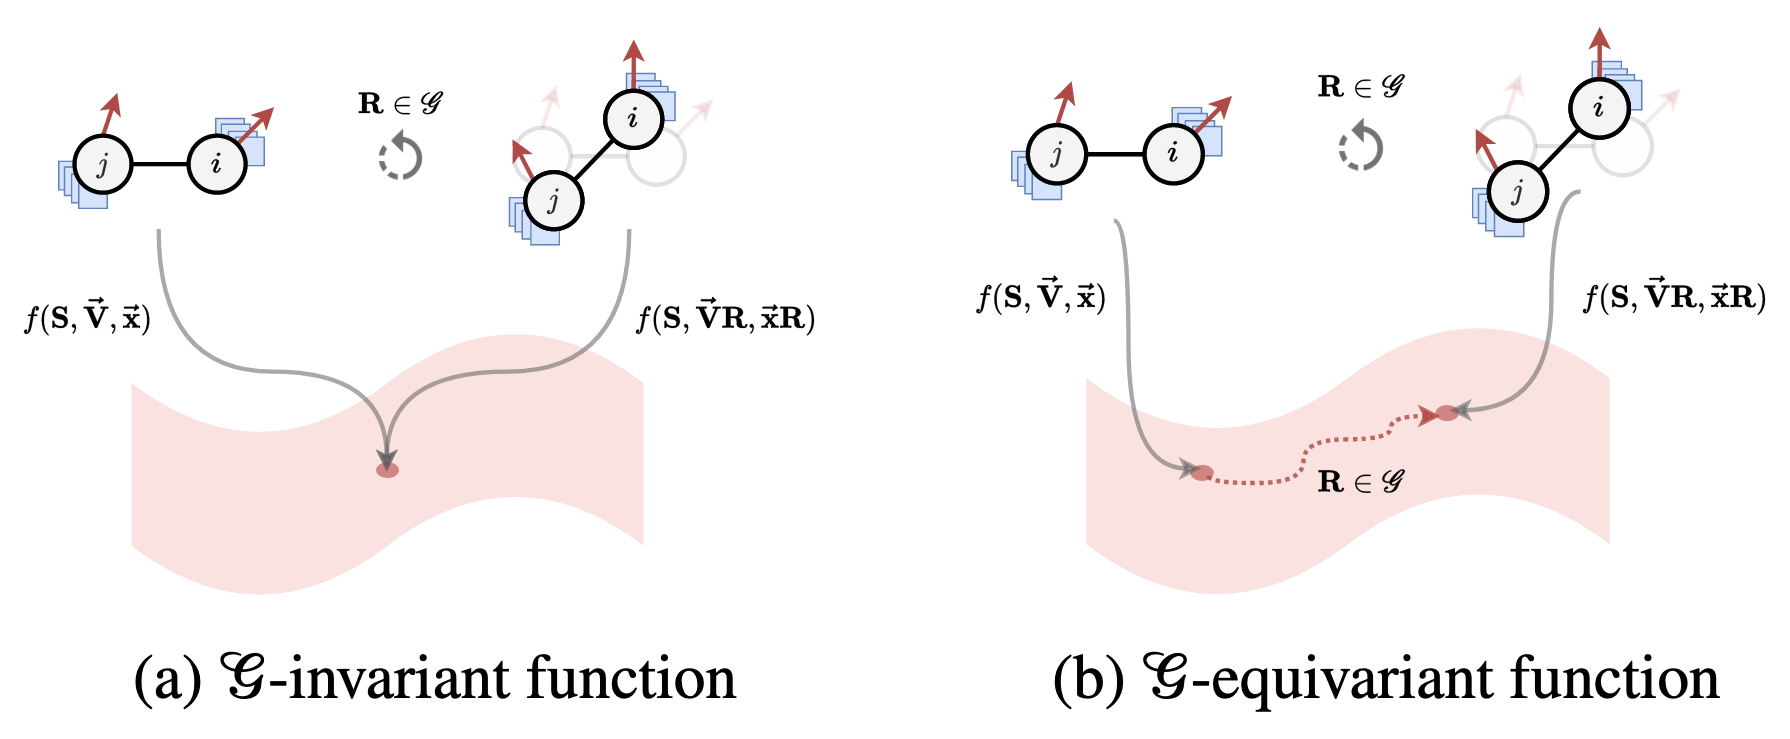
\includegraphics[width=0.8\textwidth]{Figures/2_Theory/invariance_equivariance.png}
    \caption{Invariance and equivariance. This figure was taken from \citep{duvalHitchhikersGuideGeometric2024}.}
    \label{fig:invariance_equivariance}
\end{figure}



\subsection{Equivariant graph neural networks}
In the previous section, we emphasised the importance of implementing invariance and equivariance in \acp{gnn}. In general, the field of geometric \acp{gnn} applied to computational chemistry problems is still in its early stages, since the first models were introduced around 2018, as shown in Figure~\ref{fig:equivariant_gnns}~A.

Nevertheless, the field is rapidly developing, with new architectures being proposed that advance the state of the art. These architectures achieve better performance in learning the intricacies of the potential energy surface while also scaling to systems containing millions of atoms~\citep{musaelianLearningLocalEquivariant2023}.

In this section, we focus on the general pipeline of geometric \acp{gnn}, and on the NequIP~\citep{batznerE3equivariantGraphNeural2022} neural network in particular, which stands for Neural Equivariant Interatomic Potential. The general pipeline of geometric \acp{gnn} is shown in Figure~\ref{fig:equivariant_gnns}~B.

Broadly speaking, the entire workflow can be divided into three main steps:
\begin{enumerate}
    \item Create the atomic representations.
    \item Learn the embeddings of the atomic representations.
    \item Predict the desired output property, such as the total energy or forces.
\end{enumerate}

\subsubsection{Atomic representations}
Before learning atomic representations, the network constructs an input graph from the given atomic coordinates, i.e., a point cloud. Atoms are treated as nodes, and edges are formed between atoms that lie within a specified cutoff radius. This radius defines the local environment of each atom and is crucial for ensuring that the network processes only physically meaningful interactions. To ensure a gradual change in interaction strength, a smooth cutoff function is often employed. It has the following form:

\begin{equation}
    A_{ij} = \begin{cases}
    \frac{1}{2}\left(\cos\left(\frac{\pi d_{ij}}{c}\right) + 1\right) & \text{if } d_{ij} \leq c \\
    0 & \text{otherwise}
    \end{cases}
    \label{eq:smooth_cutoff}
\end{equation}

Here, $d_{ij} = ||\vec{x}_i - \vec{x}_j||$ is the distance between atoms $i$ and $j$, and $c$ is the cutoff radius. The cutoff function smoothly transitions from 1 to 0 as the distance approaches the cutoff, ensuring that interactions are considered only within the specified range. This function is typically chosen to be continuous and differentiable, such as a cosine or polynomial function, to avoid discontinuities. The choice of cutoff radius is critical, as it determines the size of the local environment considered by the network. A cutoff that is too small may lead to the loss of important long-range interactions, while one that is too large may introduce noise and increase computational cost.

When working with periodic systems, \acp{pbc} must be respected during graph construction. Therefore, adjacent unit cells are considered within the cutoff distance to ensure that atomic environments are correctly represented.

Alongside the geometric information, usually encoded as distance-based features, each atom is assigned a type-dependent feature, often implemented as an atomic embedding vector. In addition to pairwise distances, some architectures incorporate angular information or more complex symmetry functions to capture higher-order geometric correlations. Together, these inputs form the basis of the graph on which the neural network operates.

\begin{figure}[t!]
    \centering
    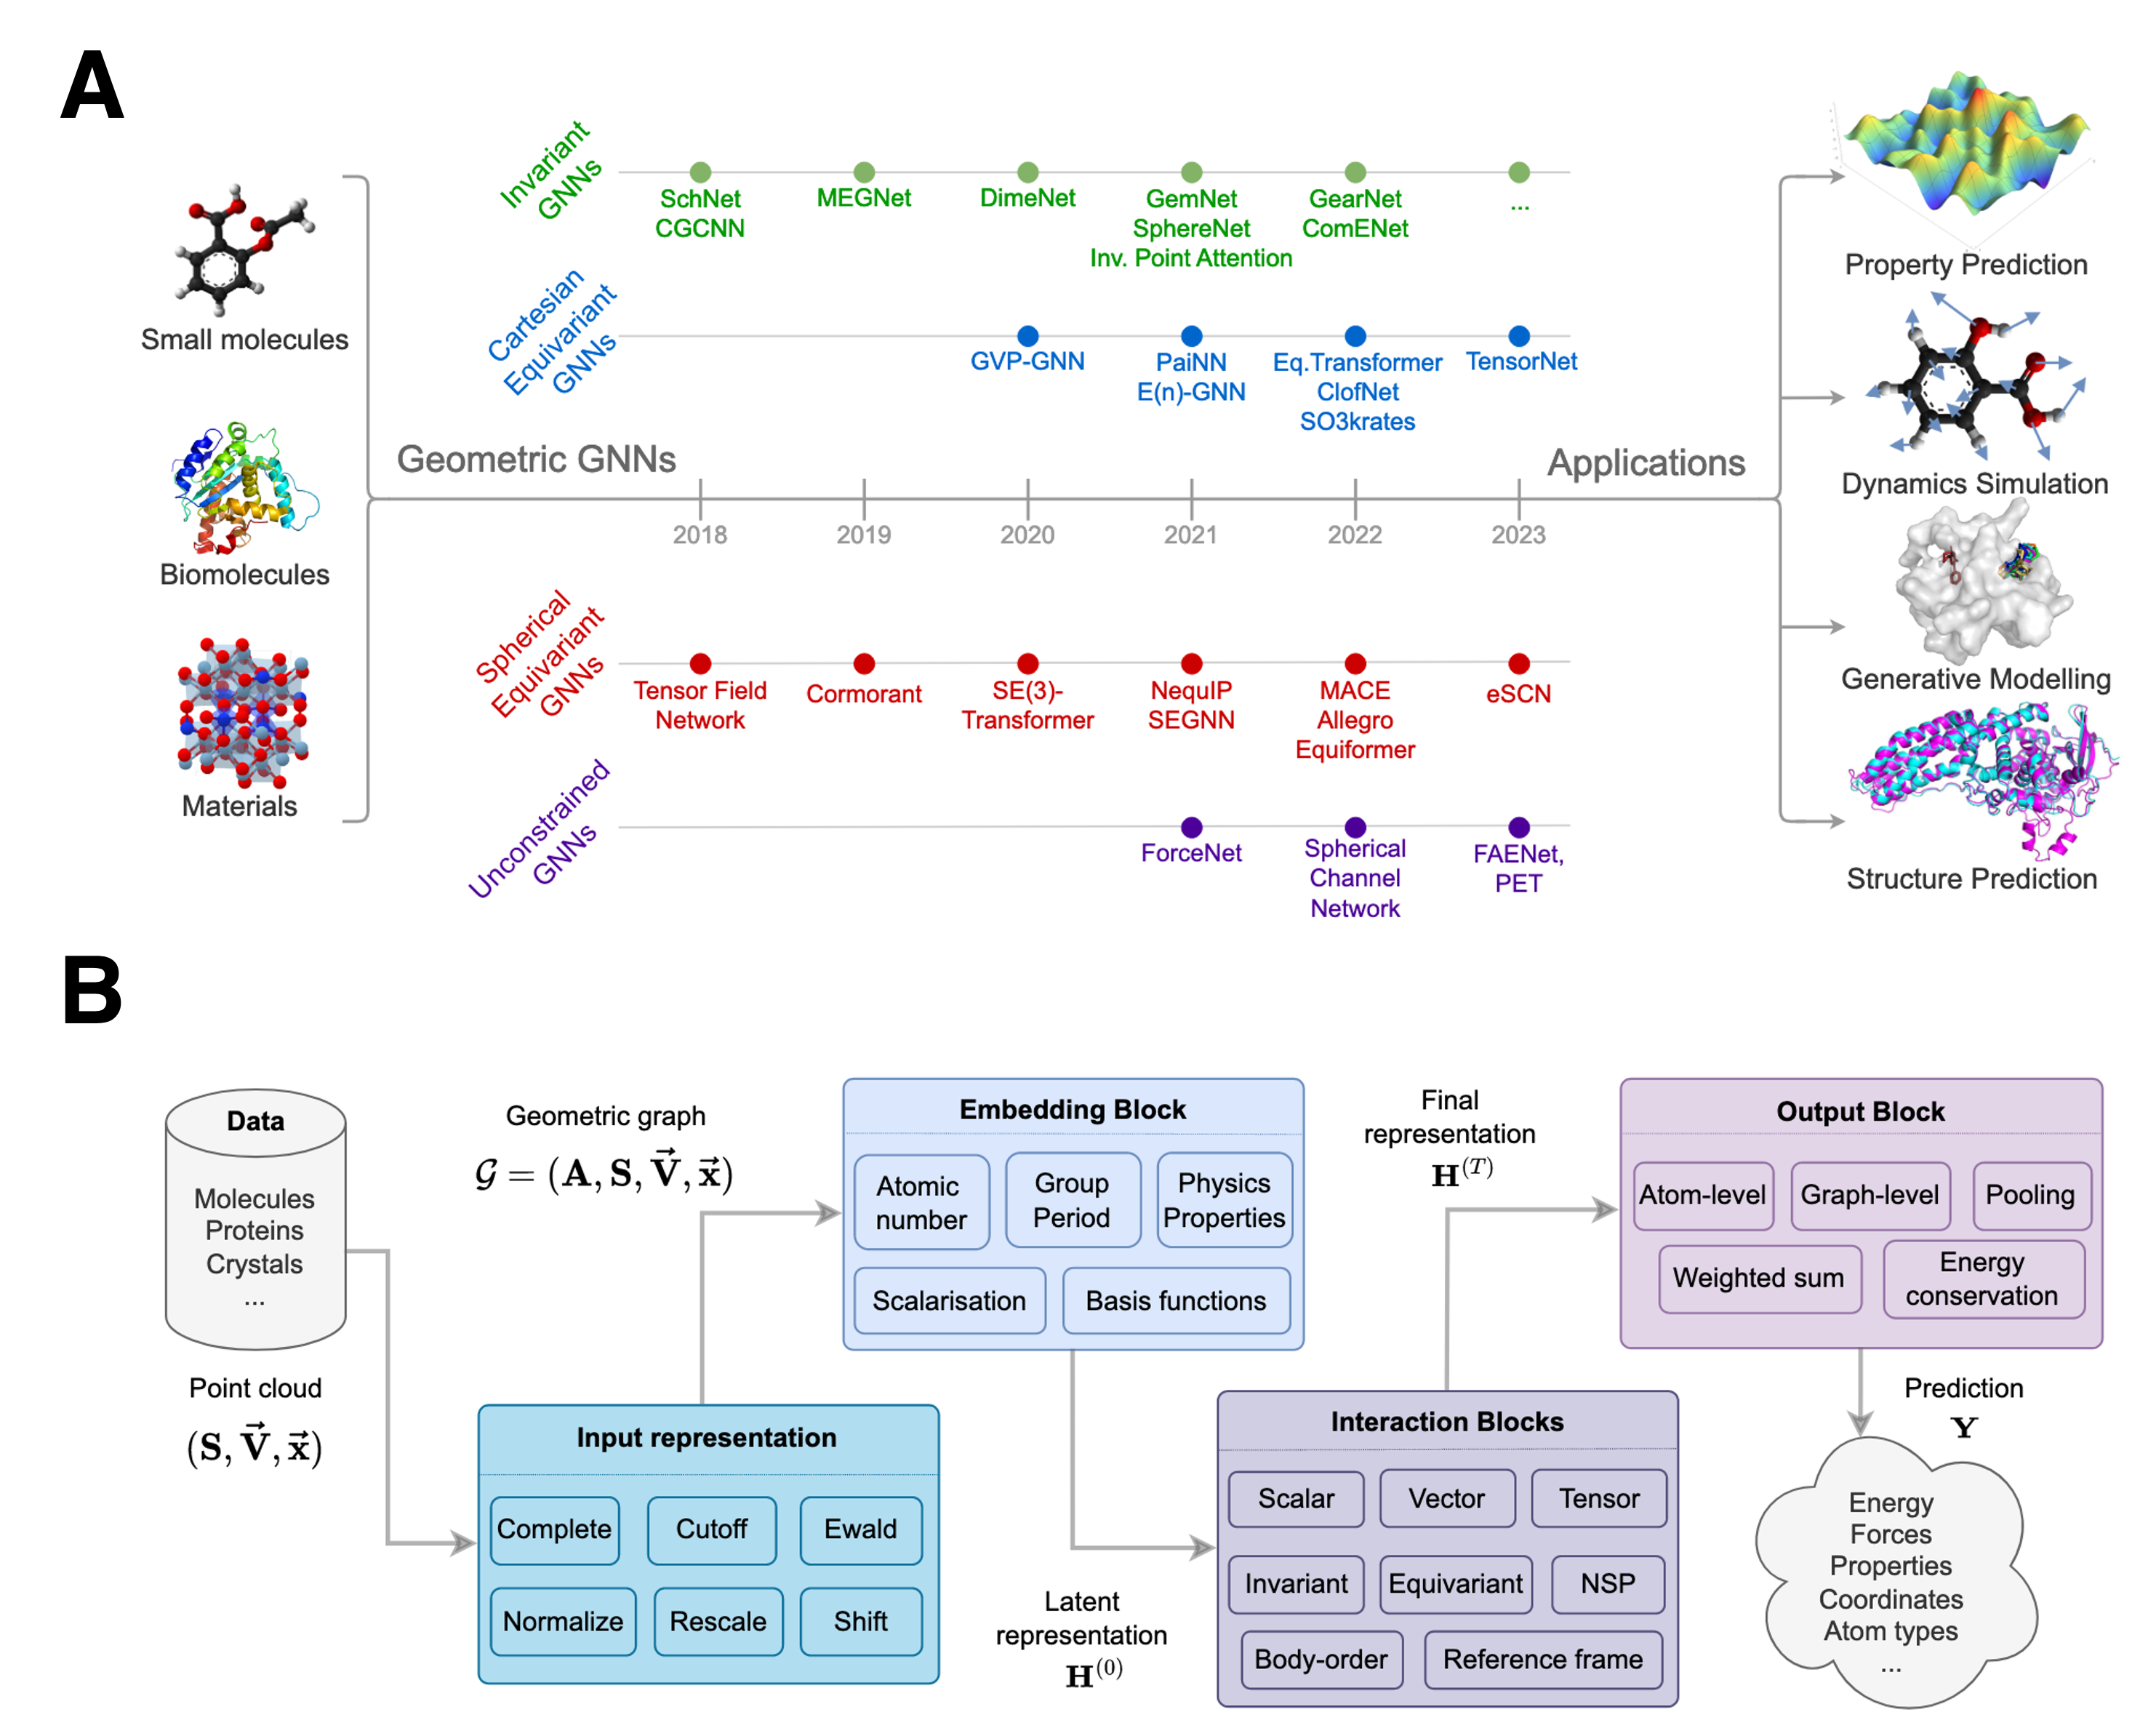
\includegraphics[width=0.9\textwidth]{Figures/2_Theory/equivariant_gnns.png}
    \caption{(A) The timeline of the development of geometric \acp{gnn} aimed at computational chemistry problems. (B) A general architecture of geometric \acp{gnn}. This figure was reproduced from \citep{duvalHitchhikersGuideGeometric2024}.}
    \label{fig:equivariant_gnns}
\end{figure}

\subsubsection{Embedding and interaction blocks}
Once the input features have been defined, the network proceeds through an initial embedding layer. This layer maps the input features into a latent space, which may consist of scalars, vectors, or higher-order tensors $\ell$, depending on the network’s level of geometric complexity. For instance, in NequIP, the input features are mapped into spherical tensors $\ell$ that are irreducible representations of $SO(3)$ thanks to the e3nn library \citep{geigerE3nnEuclideanNeural2022}, ensuring rotational equivariance, while translational invariance is built in by using relative positional features. In other words, the embedding layer constructs the initial learnable atomic representations that will be refined by the subsequent layers of the network.

The core of the network comprises a series of interaction, or message-passing, blocks. Within each block, nodes aggregate both scalar and vector information from their neighbours, often using edge features such as relative positions or spherical harmonics to guide the update. The aggregated messages are then passed through neural network layers. As a result, each node's feature vector is updated in a way that preserves the geometric structure of the system. By stacking multiple interaction blocks, the network gains the capacity to capture complex many-body interactions. Each layer builds upon the features extracted by the previous one, allowing the model to learn increasingly rich representations of atomic environments.

\subsubsection{Output block}
The final stage of a geometric \ac{gnn} involves translating the atomic representations, refined by the embedding and interaction blocks, into physically meaningful quantities, such as the total energy of the system. This quantity is typically obtained as a sum over per-atom contributions, a strategy that ensures permutation invariance with respect to atomic indexing.

To derive atomic forces, two main approaches can be used: either predicting them directly or utilising automatic differentiation. In the latter case, forces are computed as the negative gradient of the predicted energy with respect to atomic positions using automatic differentiation as implemented in modern deep learning libraries. This approach ensures that the forces are conservative and thus obey the fundamental law of energy conservation. Moreover, since the model is constructed to respect geometric symmetries, the resulting forces are also equivariant under rotations and translations.

Thanks to the incorporating the physics-inspired features and symmetry constraints, the output of the network provides physically meaningful predictions of both total energy and atomic forces.